\chapter{Control System}

The implementation process of a control system is focused on existing independently modules and underlying features in the software. The stepwise procedure for this assignment was to take on the challenge of understanding the different modules and fuse these modules to a more unified solution. A dedicated and intuitive GUI for the control system was wanted. The purpose is to provide a more overall impression of an autonomous system to simplify further aid to test and demonstrate future implementation.


\section{Earlier Design Choices}

In the previously work done by students, independent modules were designed to have a control interface that was just suitable for their implementation objectives. Therefore, the intention of the interfaces does not represent the final purpose of the modules. In the current version of GeoMod, some modules involve going through a sequence of associated modules for usage and testing. One finds again that all modules have their own control interface,  which can lead to multiple frames appearing on the monitor. It can, therefore, be difficult to keep track of each interface and simultaneously wasting monitor space. Again, the functionality of these modules could be limited because it was developed and tested independently.

\label{chap:example}
The panel seen in \Cref{fig:controlpanels} (left) is the main menu and the first frame that is displayed when running GeoMod. This panel shows a good example of how modules accessed through a GUI and how it looks like currently. Let us take an example of how the procedure in GeoMod for visualising and controlling a geometric model of a triangle. The first step is to run the software GeoMod. The main menu will then appear. Subsequently, clicking on the button labelled camera on the main menu, opens the viewport seen previously in \Cref{fig:viewport} and a corresponding GUI for camera control. All the models mention beforehand in \Cref{chap:model} will by default be rendered (over each other) on the viewport. To further move the triangle, one needs to go back to the main menu frame, and click on the button with the label triangle. Like many of the other models, a new panel corresponding to the chosen model appear. From the new the panel, clicking the move button opens up the control panel for translation and rotation of the triangle, like the one seen earlier on \Cref{fig:controlcube}.

\begin{figure}[ht]
    \centering
    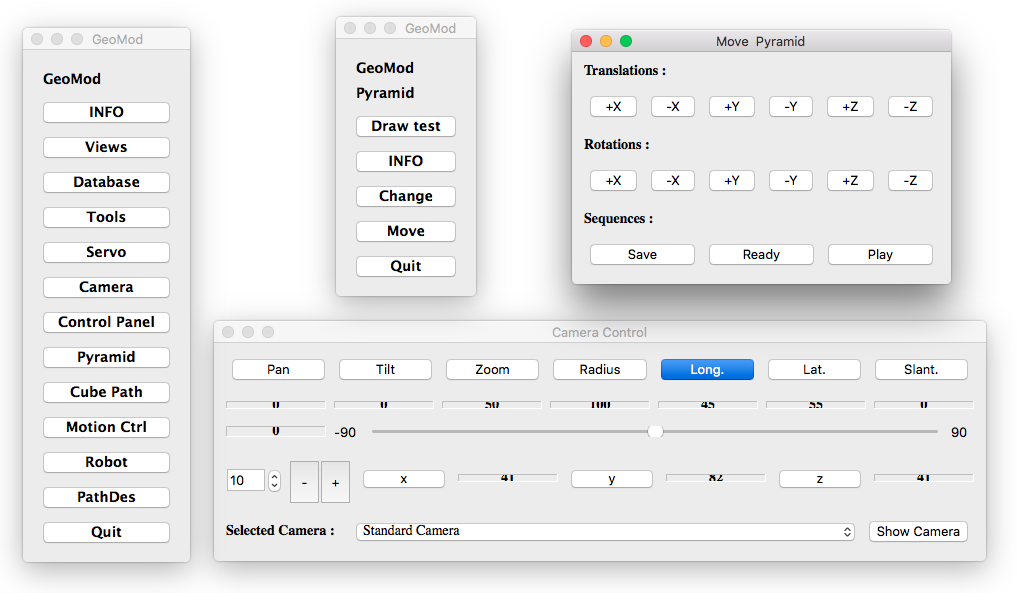
\includegraphics[height=8cm]{images/example_control.png}
    \caption[Control panels]{Left: Main Menu, top-middle: Model menu, top-right: Model control panel, bottom-right: Camera control panel}
    \label{fig:controlpanels}
\end{figure}

This example is meant to illustrate how messy and unintuitive this setup is, for something that should be somewhat straightforward to do. Notably, involving simultaneously control of multiple models would cause a headache. Not only is the main menu starting unnecessary long, but many of the buttons such as Pyramid and Cube Path are redundant as the graphical interfaces for those objects are the same. A clean up of redundancy and a structure for the graphical user interface is emphasised.

\section{Graphical User Interface}

In software development, the visual composition and behaviour of a graphical user interface is an essential part of the human-machine interaction. The GUI is meant to enhance the usability of the user and the underlying logical design of the software \cite{gui}. Qt simplifies much of the process of developing a GUI by providing graphical elements such as buttons, sliders, text, labels etc. These widgets are inherent from a class in Qt called QWidget \cite{qwidget}. In addition, Qt provides an easy way to structure widgets and communication between them. Qt's callback technique called Signal \& Slots, offers an automatic calling method produce from user interactions with widgets, which have been useful in the development of a graphical user interface \cite{signalslots}. The great thing about Qt, regarding GUI, is that it automatically uses the native graphical style (\Cref{fig:qstyle}) of the operating system it runs on. The advantage with a native theme is that users of the application do not need to get accustomed with a new design. They will be more comfortable with something they already know, as simplicity offers the best user experience of the functionality of an application. On the other hand, it is not guaranteed that the GUI is the same when ran on different operating systems. An example on this can be seen from camera control panel in \Cref{fig:controlpanels}, where the frame around the digits label is too small and narrow when ran on Mac operating system. That particular panel was implemented on a Linux operating system from a previously project. A customised design created primarily for the application can solve this uncertainty as all the operating systems are using the same theme style. Again, this requires a lot of time and works designing a theme from scratch as one also need to update the theme with new functionality added.

\begin{figure}[ht]
  \centering
  \subfloat[Windows]{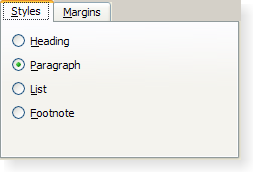
\includegraphics[width=0.3\textwidth]{images/windows.png}\label{fig:f1}}
  \hfill
  \subfloat[Linux]{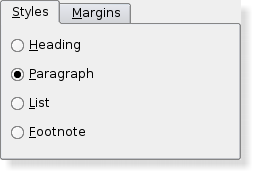
\includegraphics[width=0.3\textwidth]{images/linux.png}\label{fig:f2}}
  \hfill
  \subfloat[Mac]{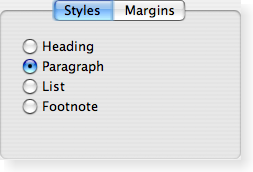
\includegraphics[width=0.3\textwidth]{images/mac.png}\label{fig:f3}}
  \caption[Natives operating system styles \cite{qstyle}]{Natives operating system styles \cite{qstyle}}
  \label{fig:qstyle}
\end{figure}


\section{Control Panel}

The objectives of the assignment (\Cref{chap:objectives}) explicitly tells to establish a control system for vehicles and tools. Thus the focused will be to adopt and utilise much of the implemented mechanics regarding the transformation control. By developing an overall control system, an arrangement of all future applicable functions have to be taken into consideration as best as possible. The GUI will be developed under the macOS operating system corresponding with macOS natives theme style.

Before implementing the control system, two main concerns needs to be thought about. What do we wish to govern? What areas of needs occurs? To the first question, the assignment emphasised on model and path control with the use of forward and inverse kinematics. In this project, an emergence of interest for the camera control arise. Like models and paths, the virtual camera consists of a basis related to the world space.  But unlike models and paths, cameras are moved in spherical coordinates that suit for its purpose. It is beforehand implemented a control panel for the camera with options to add more cameras and change viewport to a specific view of interest. Hence, this was taken into consideration for the implementation of the control system. Note that even if the camera control was relevant for the control system, an implementation of its usage was not the priority as it was outside the scope of the given assignment. However, the implemented GUI for the control system can also be applied to the cameras in future development. For the second question, it is important to know the intentions and usage of the various functions of the users. With that in mind, a graphical user interface can develop to fit the use of the users. Another important factor when designing a GUI is how organised and structured it is, to get sufficient overview of the system. As probably understood from the example in \Cref{chap:example}, overflow of framess and senseless procedure makes it complicated and clueless on how the system works.

\begin{figure}[ht]
    \centering
    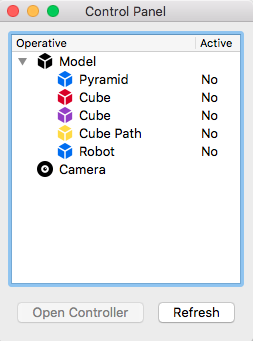
\includegraphics[height=6cm]{images/control_overview.png}
    \caption[Control overview panel]{Control overview panel}
    \label{fig:ctroverview}
\end{figure}

The idea behind the new design of the GUI was that each object should have its own control frame based on the same GUI. This approach makes it flexible to manage various types of objects simultaneously. As this method could result in an abundance of frames covering the monitor, a GUI with the overview of objects was created to prevent losing track of active frames. Not only was it easier to access the specific object, but provides an overview of the available object in the system. This fits very well regarding dynamic linking of new objects in an autonomous system. Pre-made models are currently instansiated hard-coded in the software and then added to a list of models. The same principle can be applied when adding dynamically, as long the model is added to the list of models. By accessing this list, the model's properties can then be controlled. 

An alternative design that was considered was only to have one frame as a "master" control interface over the objects. One could choose an object to control, for instance from a list within the "master" frame. This makes it, among other things, easier to keep track of within several different frames and applications. The setback of this method compromises the freedom to adapt composition of frames when working with multiple objects efficiently. 

The control overview panel seen in \Cref{fig:ctroverview} can be accessed through the main menu by clicking the button labelled Control Panel.  Controllable objects have been categorised with the corresponding symbols in the control overview panel. The symbol is created as icons from images added into Qt. The use of symbol and colours is of help to easier differentiate which control panel represents the controlled object. Note that "Cube Path" is temporarily categorised as a model due to the similar current state of behaviour.

\begin{figure}[ht]
    \centering
    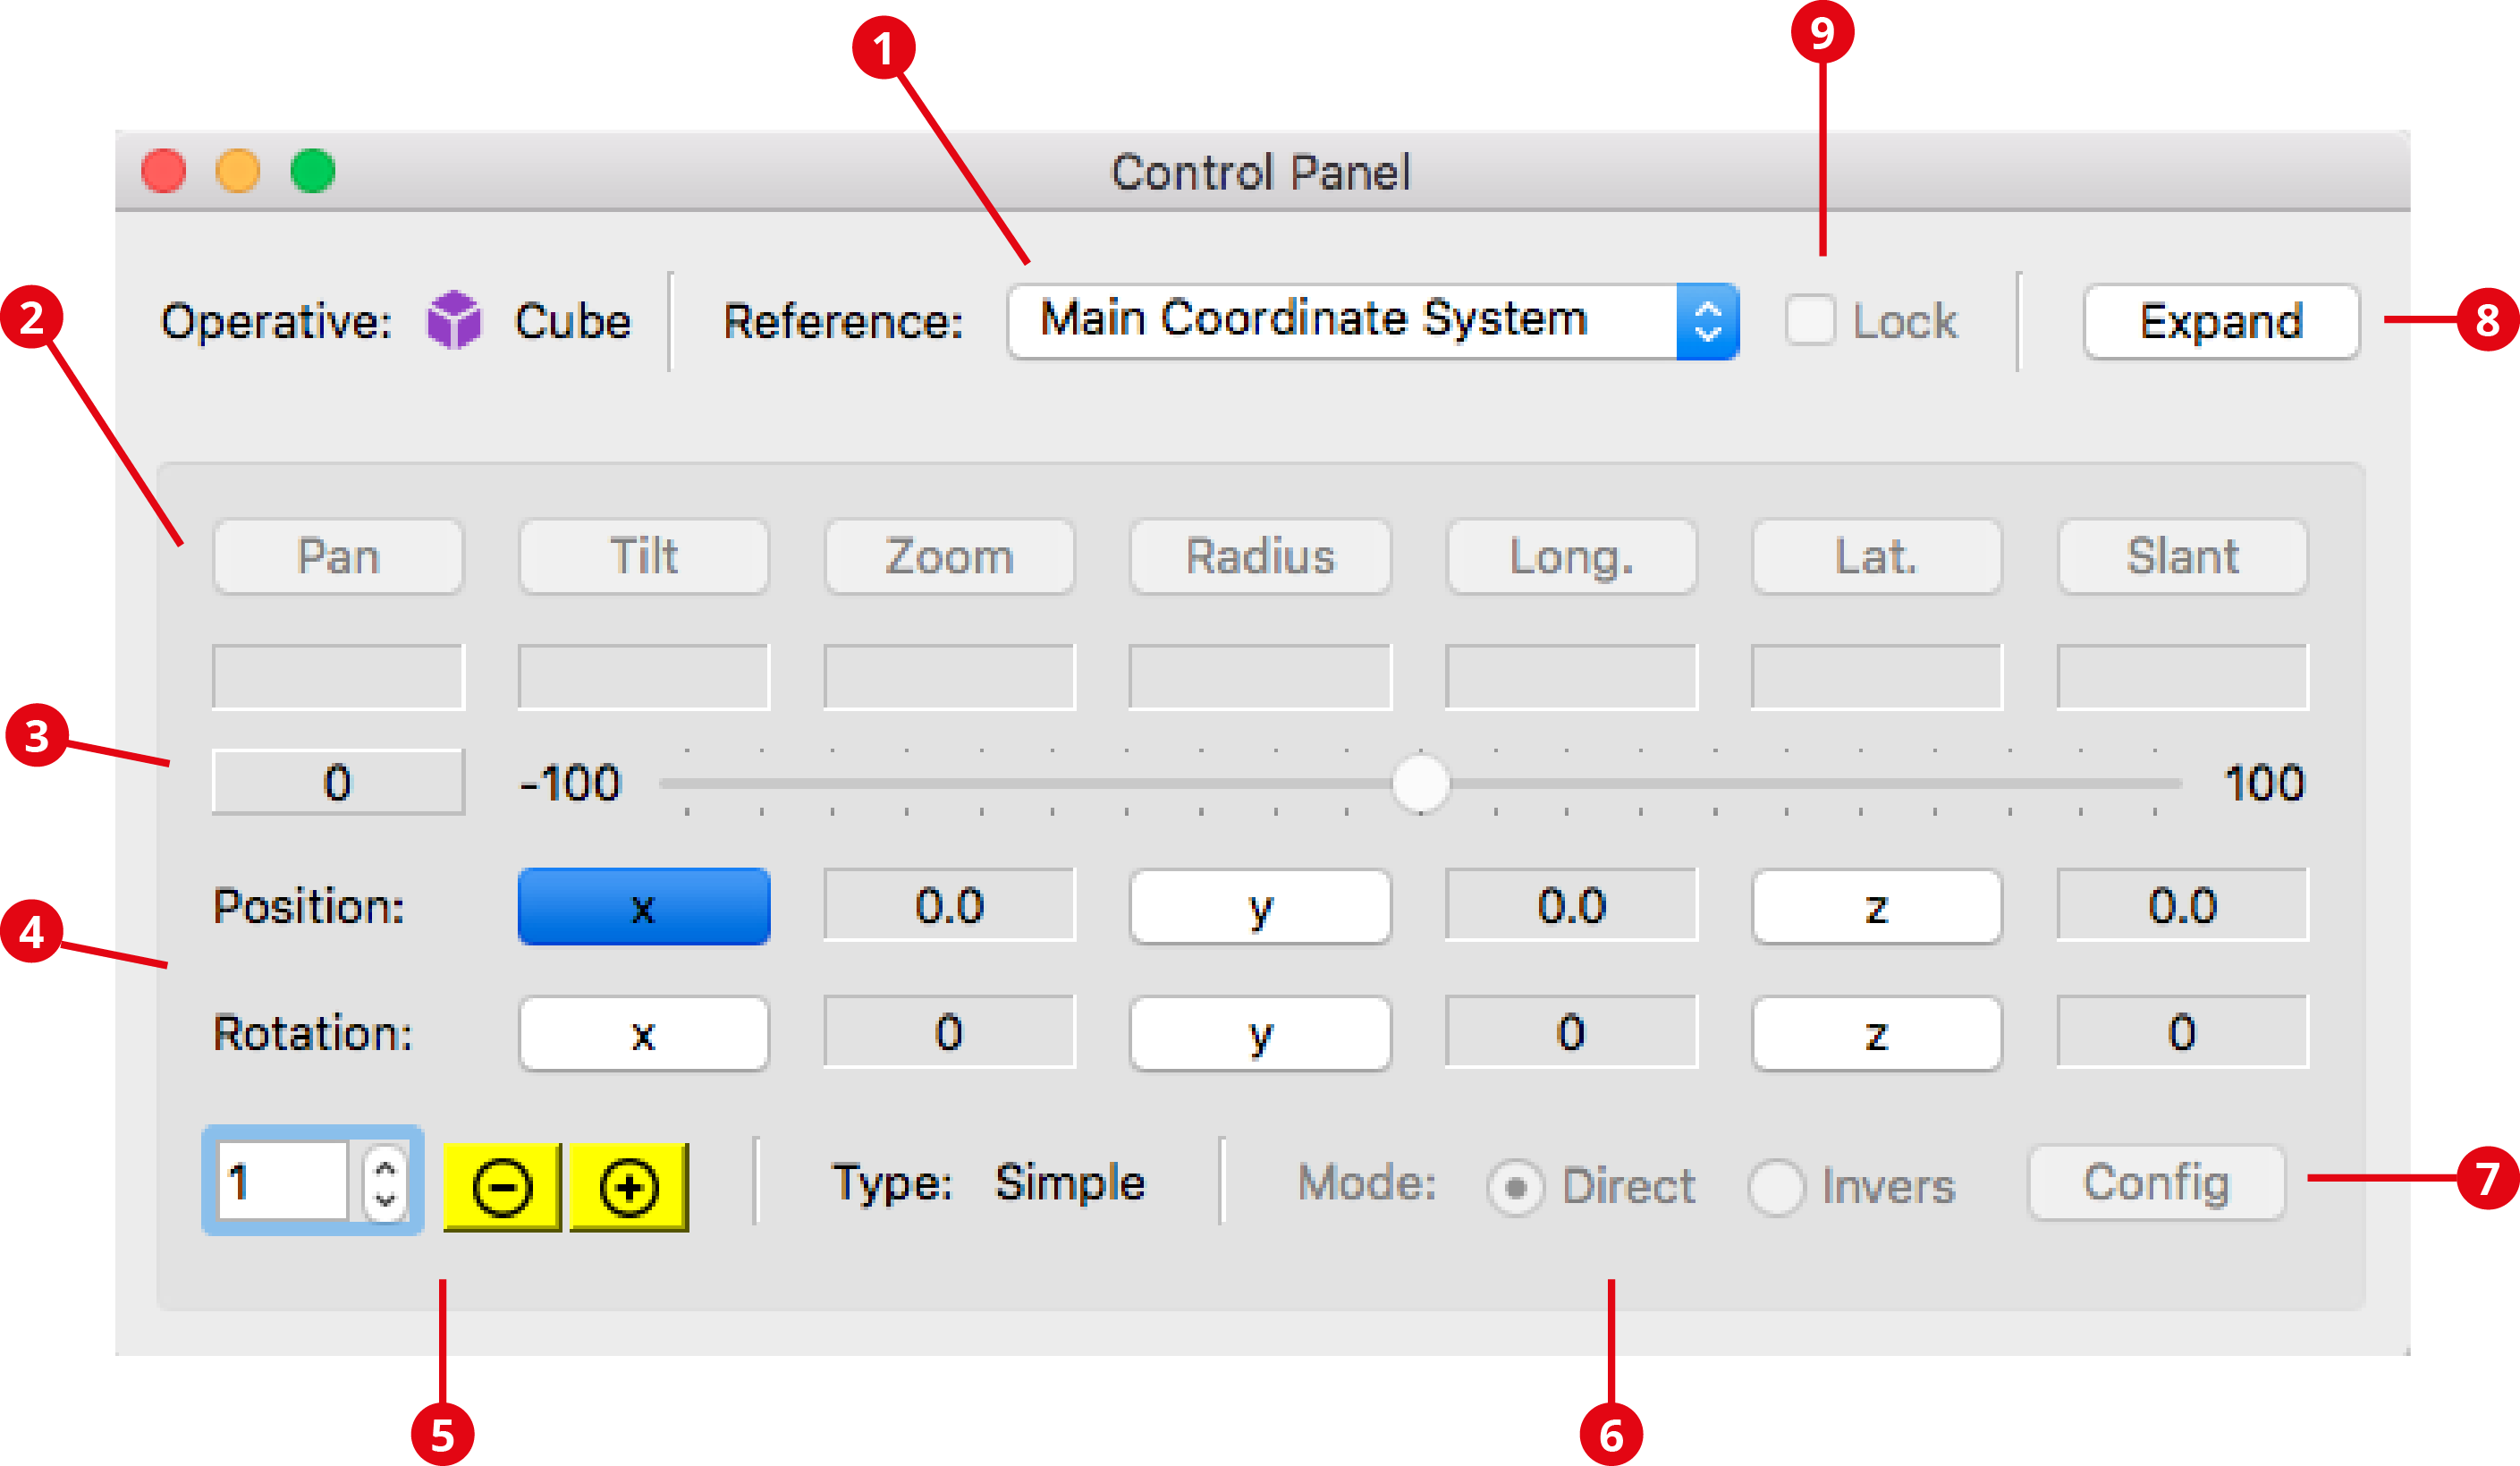
\includegraphics[height=8cm]{images/general_control_nr.png}
    \caption[Control model panel]{Control model panel}
    \label{fig:ctrgeneral}
\end{figure}

The new control GUI for models is presented in \Cref{fig:ctrgeneral}. This interface will look about the same for all models. Some control options are limited depending on the properties of the model. Similarities between this interface and the camera control interface in (figure) can seen. After guidance from the supervisor, the control ability of the camera should be beneficial in use of vehicle and tools for spherical motion. Capacity to move in spherical coordinates opens opportunities for future development of the software. Another significant advantage of this design is that the interface can also substitute the existing control interface for cameras. Based on the old control interface, much improvement had to be done visually and in the underlying code structure. Visualising position and orientation data on the model were something that was missed previously, and regarded as a helpful feature. The values of interest were specified by a method of the supervisor.  It was also aspired to be able to customise button in the form of colour to distinguish the importance functions. One might think that setting another colour on a button would be rather straightforward, but it turns out doing so would reset the stylesheet of that particular button. This means losing the native theme regarding colour and feature properties such as round-corner, size, hovering effect, clicking effect, etc. A simple and effective solution was using an image as the icon for the button. This way the native theme could be kept throughout the different operating systems without setting the properties manually. The GUI have been tested to some extent on a Windows and a Linux operating system. The result so far shows a feasible GUI on both operating systems with no unfortunate design issue. 


A summarise of the functions in the GUI will be presented under, to the number indication in \Cref{fig:ctrgeneral}.
\begin{enumerate}
\item Model movement is related to the chosen reference system. Default on the main coordinate system (world space)
\item Choose of control for movement or rotation in spherical coordinates (in the present not a implemented function and deactivated)

\item Slider control for a smooth and consistent transition (temporarily hard-coded to have an incremental value of 0.1)

\item Choose of control for movement or rotation along the three Cartesian axes.

\item Select incremental value. Increase or decrease by selected value for movement or rotation from the control options in 2. or 4. Remember the last selected value from the associated control options in 2. and 4.

\item Choose to control the model with forward or inverse kinematics. Forward kinematics is selected as default. This function is deactivated for simple models, seen from "Type". The only "complex" type who can use this function, is the serial manipulator model called "robot".

\item Corresponding to 6., only active for the type complex. This function enables the use of the associated control interface followed by the model.

\item Expand the current frame for joystick mode (\Cref{fig:joystick}).

\item Deactivated for the main coordinate system. Enables to lock on other references, such as a path or a model. When locked, the model will move accordingly to the locked reference.
\end{enumerate}

\begin{figure}[ht]
    \centering
    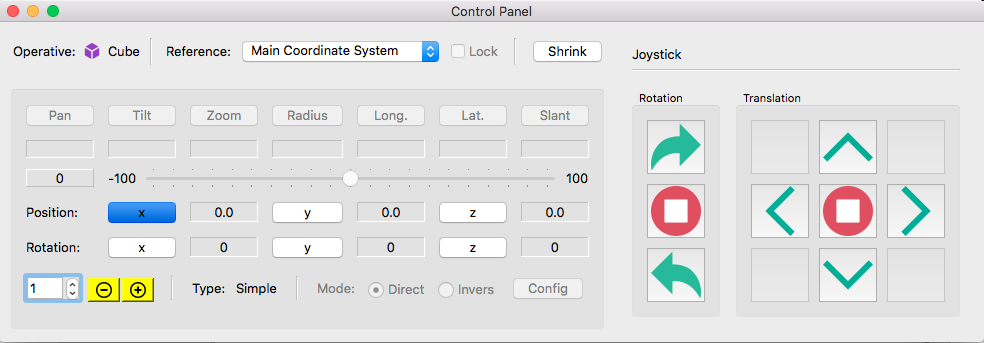
\includegraphics[height=5cm]{images/Joystick.png}
    \caption[Expanded panel for joystick mode]{Expanded panel for joystick mode}
    \label{fig:joystick}
\end{figure}

The expandable panel from \Cref{fig:joystick} was designed as a request to control with the input from a joystick device \cite{joystick}. The GUI for joystick mode is currently a visualise mock-up for future development to utilise and have no functions as of yet.

\section{Frame of reference}

In this implementation of the control system, the connection between the selected model and a chosen reference system had to be developed. The accessible references were based on the basis given from paths, models and the world space. By default, the basis of a model is defined by an offset and an orientation vector relative to the world space. In this case, the frame of reference is the world space. From this, it was reasonably straightforward to change the offset and orientation vector to be relative to the chosen reference of a model space. Adding this function enables a model to switch between references to follow. This allows vehicles and tools to follow given reference system as long it a can be retrieved from the system statically or dynamically. But what if the reference system is not static? The tracked reference system of a vehicle can, for instance, be in motion. A solution to this problem was using the publish-subscribe pattern described in \Cref{chap:pubsub}. This pattern is similar to that of another called Observer pattern \cite{observer_pattern}. But the main difference is that in the observer pattern the sender and the receiver are directly known to each other, which cause dependencies that are not wanted. Another undesirable action is that the receiver is asking the sender if anything has changed. For an autonomous system, adding and removing models dynamically, the publish-subscribe pattern is suitable for this purpose with regards to decoupling \cite{decoupling}. The followed reference system notify if changes occur, those models who are tracking the particular reference will be updated automatically.  

\begin{figure}[ht]
    \centering
    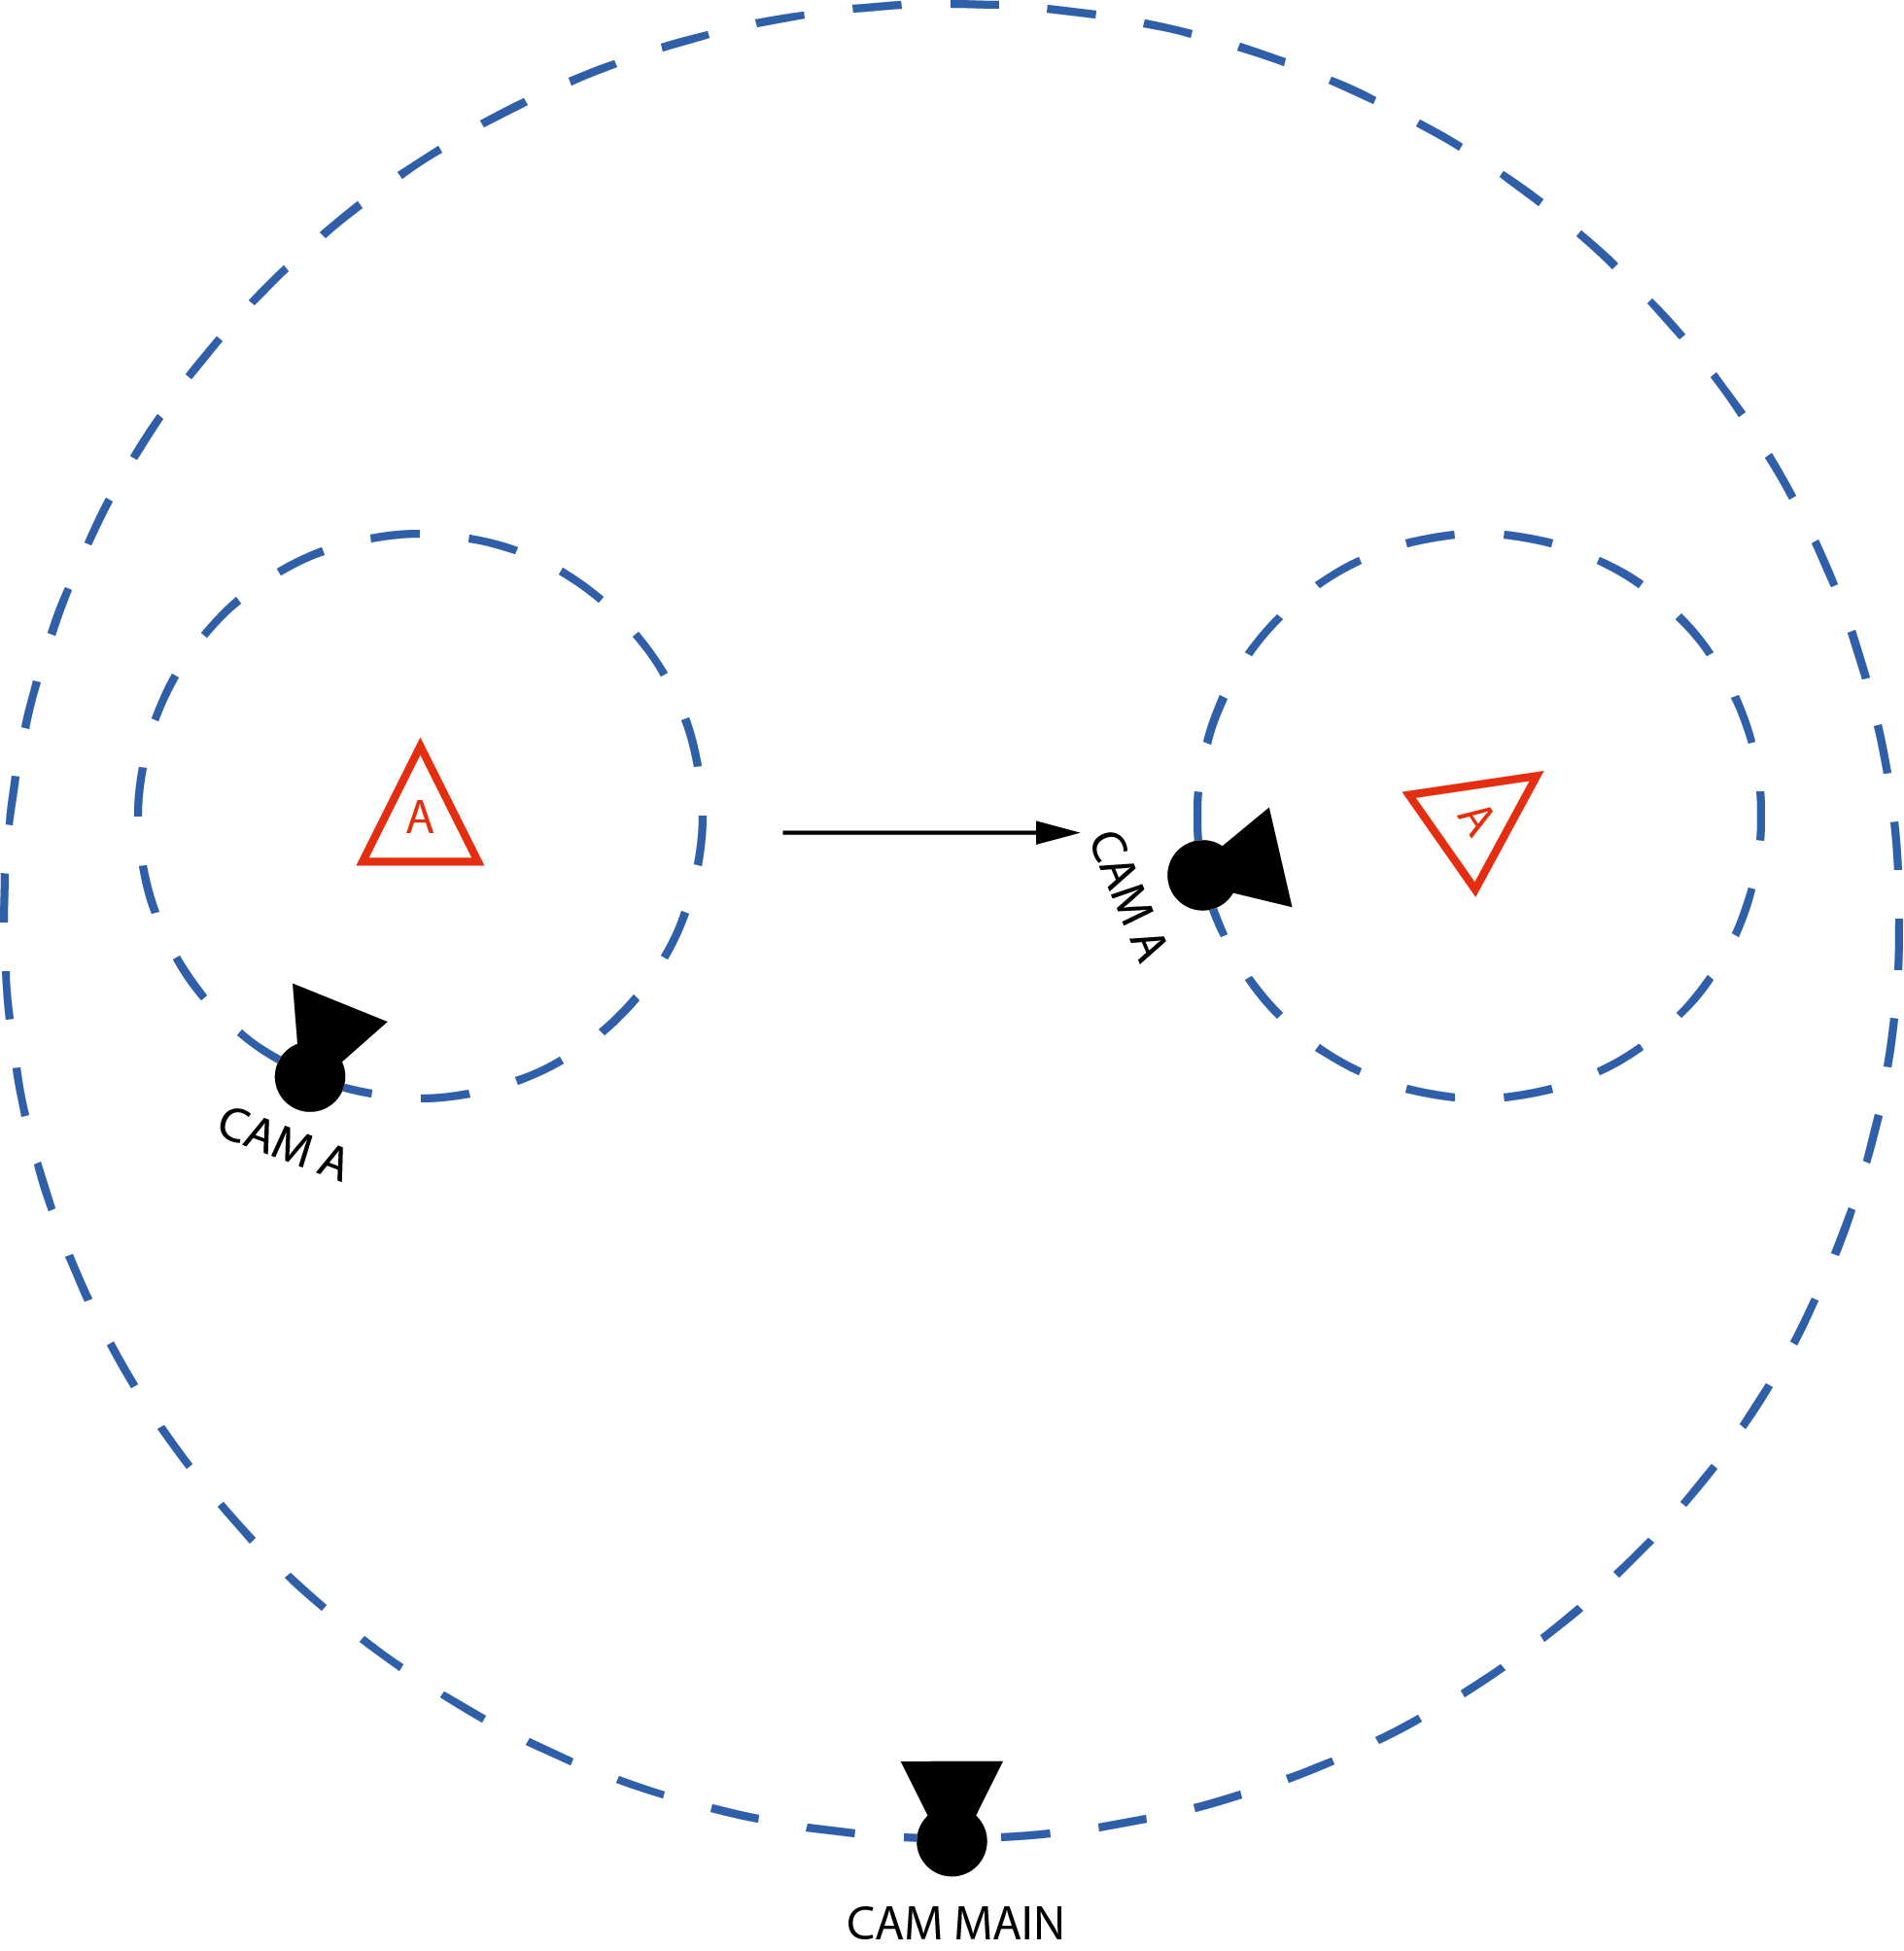
\includegraphics[height=7cm]{images/cam_ex.png}
    \caption[Camera locked on a model]{Camera locked on a model}
    \label{fig:cam_ex}
\end{figure}

This functionality can also be use for cameras and seen as a highly valued feature for future development. The \Cref{fig:cam_ex} illustrate an example for practical usage. In the example, the CAM MAIN is usually the main viewport in the software. CAM A is locked on the model A from a preferred angle, then model A move and rotate to another direction. CAM A is updated with the movement and has kept the same view angle on the model. The viewport can be changed between CAM MAIN and CAM A. This example also show how the system can be used for surveillance of autonomous vehicles. 